% Préambule commun des schémas TikZ (compilés séparément par construire_figures.py)
\documentclass[tikz,border=3pt]{standalone}
\usepackage[T1]{fontenc}
\usepackage[utf8]{inputenc}
\usepackage{lmodern}
\usepackage{amsmath,amssymb}
\usepackage{bm}
\usepackage[american,siunitx,straightvoltages]{circuitikz}
\usetikzlibrary{arrows.meta,positioning,calc,decorations.pathmorphing,
  decorations.markings,decorations.pathreplacing,patterns,shapes.geometric,
  shapes.misc,shapes.multipart,fit,backgrounds,3d,intersections,matrix}

\ctikzset{bipoles/length=1.1cm, amplifiers/scale=0.85, tripoles/op amp/width=1.4}

\tikzset{
  >={Latex[length=2mm,width=1.4mm]},
  every picture/.style={line width=0.6pt, font=\small},
  % schémas-blocs
  bloc/.style={draw, minimum width=1.5cm, minimum height=0.9cm, align=center,
               inner sep=3pt, fill=white},
  somme/.style={draw, circle, minimum size=4.5mm, inner sep=0pt, fill=white,
                path picture={\draw (path picture bounding box.north west)
                  -- (path picture bounding box.south east)
                  (path picture bounding box.north east)
                  -- (path picture bounding box.south west);}},
  gain/.style={draw, isosceles triangle, isosceles triangle apex angle=60,
               minimum size=8mm, inner sep=1pt, fill=white},
  bruit/.style={draw, circle, minimum size=4.5mm, inner sep=0pt, fill=white,
                path picture={\node at (path picture bounding box.center)
                  {\scriptsize$\ast$};}},
  cadre/.style={draw, dashed, rounded corners=1pt},
  cadrept/.style={draw, dash dot, rounded corners=1pt},
  fleche/.style={->},
  % mécanique
  bati/.style={pattern=north east lines, draw=none},
  ressort/.style={decorate, decoration={coil, aspect=0.4, segment length=2.2mm,
                  amplitude=2mm, pre length=2mm, post length=2mm}},
  zigzag/.style={decorate, decoration={zigzag, segment length=2mm,
                  amplitude=1.6mm, pre length=2mm, post length=2mm}},
  pivot/.style={draw, circle, fill=white, minimum size=2.2mm, inner sep=0pt},
  masse/.style={draw, fill=gray!25, minimum width=1.4cm, minimum height=0.8cm},
  cote/.style={<->, line width=0.4pt},
  axe/.style={->, line width=0.6pt},
  trait mixte/.style={dash dot, line width=0.4pt},
}

% Encastrement / bâti hachuré : \bati{(x1,y1)}{(x2,y2)} trace une ligne et ses hachures dessous
\newcommand{\bati}[3][0.18]{%
  \fill[pattern=north east lines] #2 rectangle ($#3+(0,-#1)$);
  \draw[line width=0.8pt] #2 -- #3;}

% Transducteur (deux cercles entrelacés) : \pic (t) at (x,y) {transducteur};  -> (t-o) entrée, (t-e) sortie
\tikzset{
  transducteur/.pic={\draw (-0.13,0) circle (0.24); \draw (0.13,0) circle (0.24);
    \coordinate (-o) at (-0.37,0); \coordinate (-e) at (0.37,0);
    \coordinate (-n) at (0,0.24); \coordinate (-s) at (0,-0.24);},
  bobine/.style={decorate, decoration={coil, aspect=0.7, segment length=1.4mm,
                 amplitude=1.6mm, pre length=1mm, post length=1mm}},
  sourcebruit/.style={draw, circle, minimum size=5mm, inner sep=0pt, fill=white,
                 label={[inner sep=0pt]center:$\ast$}},
  sourcecourant/.style={draw, circle, minimum size=5mm, inner sep=0pt, fill=white,
                 label={[inner sep=0pt]center:$\circledast$}},
}

% Composants compacts (pour les petits boîtiers des schémas-blocs)
\newcommand{\resistance}[2]{% de #1 à #2 (quelconque)
  \draw #1 -- ($#1!0.22!#2$) ($#1!0.78!#2$) -- #2;
  \draw[decorate, decoration={zigzag, segment length=1.5mm, amplitude=1.1mm}]
    ($#1!0.22!#2$) -- ($#1!0.78!#2$);}
\newcommand{\condensateur}[2]{% horizontal de #1 à #2
  \draw #1 -- ($($#1!0.5!#2$)+(-0.05,0)$) ($($#1!0.5!#2$)+(0.05,0)$) -- #2;
  \draw[line width=1pt] ($($#1!0.5!#2$)+(-0.05,0.14)$) -- ($($#1!0.5!#2$)+(-0.05,-0.14)$)
                        ($($#1!0.5!#2$)+(0.05,0.14)$) -- ($($#1!0.5!#2$)+(0.05,-0.14)$);}
% R // C horizontal : \RparC{(x,y)}{longueur}{écart}  (centre, longueur totale, écart vertical)
\newcommand{\RparC}[3]{%
  \coordinate (rcA) at ($#1+(-#2/2,0)$); \coordinate (rcB) at ($#1+(#2/2,0)$);
  \draw (rcA) -- ++(0.15,0) coordinate (rcA1) (rcB) -- ++(-0.15,0) coordinate (rcB1);
  \draw (rcA1) -- ++(0,#3/2) (rcA1) -- ++(0,-#3/2) (rcB1) -- ++(0,#3/2) (rcB1) -- ++(0,-#3/2);
  \resistance{($(rcA1)+(0,#3/2)$)}{($(rcB1)+(0,#3/2)$)}
  \condensateur{($(rcA1)+(0,-#3/2)$)}{($(rcB1)+(0,-#3/2)$)}}

% Schéma électrique de la carte SIS-ASSER (redessiné ; condensateurs de découplage
% des alimentations et numéros de broches omis)
\ctikzset{bipoles/length=0.85cm, amplifiers/scale=0.7}
\newcommand{\boite}[4]{\node[draw, minimum width=#2, minimum height=#3, align=center, fill=white] at #1 {#4};}
\newcommand{\suiveur}[1]{\draw (#1.-) -- ++(-0.25,0) -- ++(0,-0.45) -| ($(#1.out)+(0.25,0)$);}
\begin{document}
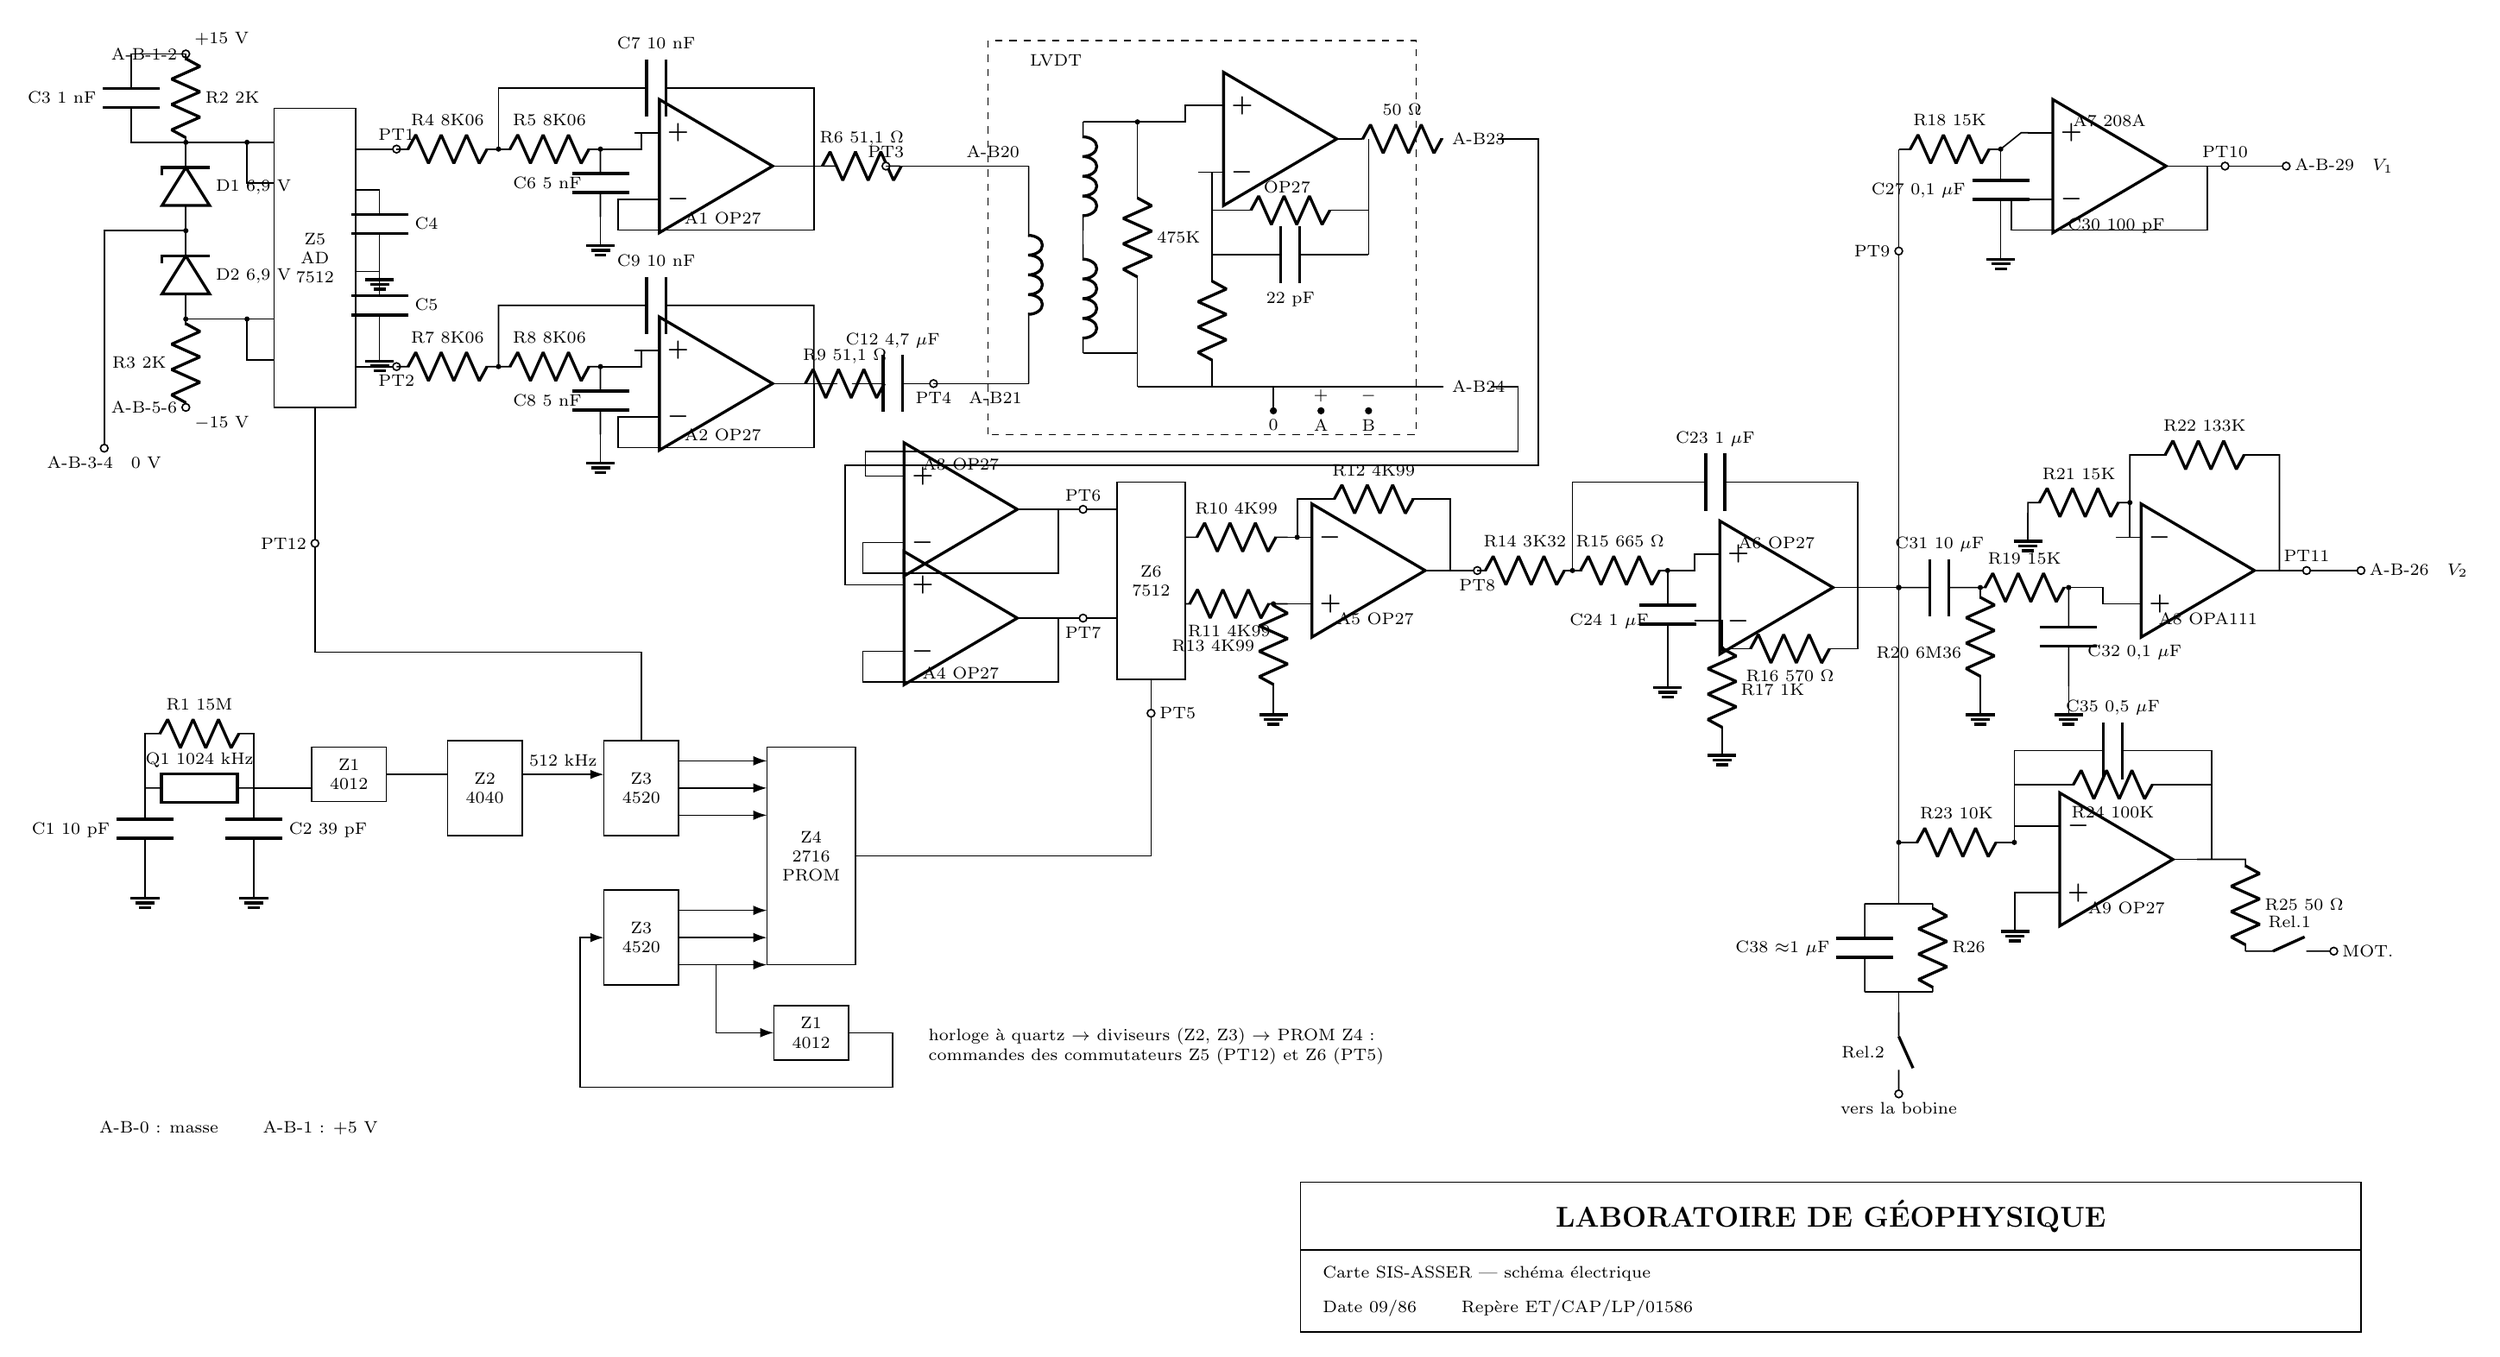
\begin{tikzpicture}[font=\scriptsize]
  % ================= A. références de tension et commutateur Z5 =================
  \draw (0.6,12.2) node[ocirc] {} node[left] {A-B-1-2} node[above right] {$+15$ V};
  \draw (0.6,12.2) to[R, l={R2 2K}] (0.6,10.9);
  \draw (0.6,12.2) -- (-0.2,12.2) to[C, l_={C3 1 nF}] (-0.2,10.9) -- (0.6,10.9);
  \draw (0.6,9.6) to[zD, l_={D1 6,9 V}] (0.6,10.9);
  \draw (0.6,8.3) to[zD, l_={D2 6,9 V}] (0.6,9.6);
  \draw (0.6,8.3) to[R, l_={R3 2K}] (0.6,7.0) node[ocirc] {} node[left] {A-B-5-6} node[below right] {$-15$ V};
  \foreach \y in {10.9,9.6,8.3} \fill (0.6,\y) circle (1.1pt);
  \draw (0.6,9.6) -- (-0.6,9.6) -- (-0.6,6.4) node[ocirc] {} node[below] {A-B-3-4 \; 0 V};
  \draw (1.9,7.0) rectangle (3.1,11.4); \node[align=center] at (2.5,9.2) {Z5\\AD\\7512};
  \draw (0.6,10.9) -- (1.9,10.9) (1.5,10.9) |- (1.9,10.3); \fill (1.5,10.9) circle (1.1pt);
  \draw (0.6,8.3) -- (1.9,8.3) (1.5,8.3) |- (1.9,7.7); \fill (1.5,8.3) circle (1.1pt);
  \draw (3.1,10.8) -- (3.7,10.8) node[ocirc] {} node[above] {PT1};
  \draw (3.1,7.6) -- (3.7,7.6) node[ocirc] {} node[below] {PT2};
  \draw (3.1,10.2) -| (3.45,10.1) to[C, l={C4}] (3.45,9.3) node[ground] {};
  \draw (3.1,9.0) -| (3.45,8.9) to[C, l={C5}] (3.45,8.1) node[ground] {};
  % ================= B. filtres de mise en forme A1 et A2 =================
  \foreach \y/\na/\ra/\rb/\cc/\cd in {10.8/A1/R4/R5/C7 10 nF/C6 5 nF, 7.6/A2/R7/R8/C9 10 nF/C8 5 nF} {
    \draw (3.7,\y) to[R, l={\ra\ 8K06}] (5.2,\y) to[R, l={\rb\ 8K06}] (6.7,\y);
    \fill (5.2,\y) circle (1.1pt) (6.7,\y) circle (1.1pt);
    \draw (6.7,\y) to[C] (6.7,\y-1.0) node[ground] {};
    \node[left] at (6.55,\y-0.5) {\cd};
    \draw (8.4,\y-0.25) node[op amp, noinv input up] (\na) {};
    \node[below] at ($(\na)+(0.1,-0.55)$) {\na\ OP27};
    \draw (6.7,\y) -- (7.3,\y) |- (\na.+);
    \suiveur{\na}
    \draw (5.2,\y) -- (5.2,\y+0.9) to[C, l={\cc}] ($(\na.out)+(0.25,0)+(0,\y+0.9)-(0,\y-0.25)$) -- ($(\na.out)+(0.25,0)$);
    \draw (\na.out) -- ($(\na.out)+(0.6,0)$);
  }
  % ================= C. LVDT et étage de tête (au niveau du capteur) =================
  \draw ($(A1.out)+(0.6,0)$) to[R, l={R6 51,1 $\Omega$}] (10.9,0 |- A1.out) node[ocirc] {} node[above] {PT3};
  \draw ($(A2.out)+(0.6,0)$) to[R, l={R9 51,1 $\Omega$}] (10.4,0 |- A2.out) to[C, l={C12 4,7 $\mu$F}] (11.6,0 |- A2.out) node[ocirc] {} node[below] {PT4};
  \draw (10.9,0 |- A1.out) -- (13.0,0 |- A1.out) node[pos=0.75, above] {A-B20};
  \draw (11.6,0 |- A2.out) -- (13.0,0 |- A2.out) node[pos=0.65, below] {A-B21};
  \draw[dashed] (12.4,6.6) rectangle (18.7,12.4);
  \node at (13.4,12.1) {LVDT};
  \draw (13.0,0 |- A1.out) to[L] (13.0,0 |- A2.out);
  \draw (13.8,11.2) to[L] (13.8,9.6); \draw (13.8,9.4) to[L] (13.8,7.8); \draw (13.8,9.6) -- (13.8,9.4);
  \draw (13.8,11.2) -- (14.6,11.2) to[R, l={475K}] (14.6,7.8) -- (13.8,7.8);
  \draw (14.6,7.8) -- (14.6,7.3);
  \draw (16.7,10.95) node[op amp, noinv input up] (T) {}; \node[below] at ($(T)+(0.1,-0.5)$) {OP27};
  \fill (14.6,11.2) circle (1.1pt);
  \draw (14.6,11.2) -- (15.3,11.2) |- (T.+);
  \draw (T.-) -- (15.7,0 |- T.-) -- (15.7,9.9);
  \draw (15.7,9.9) to[R] (18.0,9.9) (15.7,9.25) to[C, l_={22 pF}] (18.0,9.25);
  \draw (15.7,9.9) -- (15.7,9.25) (18.0,9.25) -- (18.0,0 |- T.out);
  \draw (15.7,9.25) to[R] (15.7,7.3);
  \draw (T.out) to[R, l={50 $\Omega$}] (19.1,0 |- T.out) node[right] {A-B23};
  \draw (14.6,7.3) -- (19.1,7.3) node[right] {A-B24};
  \draw (16.6,7.3) -- (16.6,6.95);
  \foreach \x/\t/\s in {16.6/0/, 17.3/A/$+$, 18.0/B/$-$} {\fill (\x,6.95) circle (1.5pt); \node[below] at (\x,6.95) {\t}; \node[above] at (\x,6.95) {\s};}
  % ================= D. prédémodulation, démodulation, filtrage =================
  \draw (12.0,5.5) node[op amp, noinv input up] (A3) {}; \node[above] at ($(A3)+(0,0.45)$) {A3 OP27};
  \draw (12.0,3.9) node[op amp, noinv input up] (A4) {}; \node[below] at ($(A4)+(0,-0.6)$) {A4 OP27};
  \draw (19.8,7.3) -- (20.2,7.3) -- (20.2,6.35) -- (10.6,6.35) |- (A3.+);
  \draw (19.9,0 |- T.out) -- (20.5,0 |- T.out) -- (20.5,6.15) -- (10.3,6.15) |- (A4.+);
  \suiveur{A3} \suiveur{A4}
  \draw (A3.out) -- (13.8,0 |- A3.out) node[ocirc] {} node[above] {PT6} -- (14.3,0 |- A3.out);
  \draw (A4.out) -- (13.8,0 |- A4.out) node[ocirc] {} node[below] {PT7} -- (14.3,0 |- A4.out);
  \draw (14.3,3.0) rectangle (15.3,5.9); \node[align=center] at (14.8,4.45) {Z6\\7512};
  \draw (14.8,3.0) -- (14.8,2.0); \draw (14.8,2.5) node[ocirc] {} node[right] {PT5};
  \draw (18.0,4.6) node[op amp] (A5) {}; \node[below] at ($(A5)+(0.1,-0.5)$) {A5 OP27};
  \draw (15.3,0 |- A5.-) to[R, l={R10 4K99}] (A5.-);
  \draw (15.3,0 |- A5.+) to[R, l_={R11 4K99}] (16.6,0 |- A5.+) -- (A5.+);
  \fill (16.6,0 |- A5.+) circle (1.1pt) (16.95,0 |- A5.-) circle (1.1pt);
  \draw (16.6,0 |- A5.+) to[R] (16.6,2.9) node[ground] {}; \node[left] at (16.45,3.5) {R13 4K99};
  \draw (16.95,0 |- A5.-) -- (16.95,5.65) to[R, l={R12 4K99}] (19.2,5.65) -- (19.2,0 |- A5.out);
  \draw (A5.out) -- (19.6,0 |- A5.out) node[ocirc] {} node[below] {PT8};
  \draw (19.6,0 |- A5.out) to[R, l={R14 3K32}] (21.0,0 |- A5.out) to[R, l={R15 665 $\Omega$}] (22.4,0 |- A5.out);
  \fill (21.0,0 |- A5.out) circle (1.1pt) (22.4,0 |- A5.out) circle (1.1pt);
  \draw (22.4,0 |- A5.out) to[C] (22.4,3.3) node[ground] {}; \node[left] at (22.25,3.85) {C24 1 $\mu$F};
  \draw (24.0,4.35) node[op amp, noinv input up] (A6) {}; \node[above] at ($(A6)+(0,0.45)$) {A6 OP27};
  \draw (22.4,0 |- A5.out) -- (22.8,0 |- A5.out) |- (A6.+);
  \draw (21.0,0 |- A5.out) -- (21.0,5.9) to[C, l={C23 1 $\mu$F}] (25.2,5.9) -- (25.2,0 |- A6.out);
  \draw (A6.-) -- (23.2,0 |- A6.-) -- (23.2,3.45) coordinate (a6m); \fill (a6m) circle (1.1pt);
  \draw (a6m) to[R, l_={R16 570 $\Omega$}] (25.2,3.45) -- (25.2,0 |- A6.out);
  \draw (a6m) to[R] (23.2,2.3) node[ground] {}; \node[right] at (23.35,2.85) {R17 1K};
  \draw (A6.out) -- (25.8,0 |- A6.out) coordinate (P); \fill (P) circle (1.2pt);
  % ================= E. étages de sortie =================
  % voie V1 (A7)
  \draw (P) -- (25.8,9.3) node[ocirc] {} node[left] {PT9} -- (25.8,10.8);
  \draw (25.8,10.8) to[R, l={R18 15K}] (27.3,10.8); \fill (27.3,10.8) circle (1.1pt);
  \draw (27.3,10.8) to[C, l_={C27 0,1 $\mu$F}] (27.3,9.6) node[ground] {};
  \draw (28.9,10.55) node[op amp, noinv input up] (A7) {}; \node[above] at ($(A7)+(0,0.45)$) {A7 208A};
  \draw (27.3,10.8) -- (A7.+ -| 27.6,0) |- (A7.+);
  \suiveur{A7} \node[below] at ($(A7)+(0.1,-0.65)$) {C30 100 pF};
  \draw (A7.out) -- (30.6,0 |- A7.out) node[ocirc] {} node[above] {PT10} -- (31.5,0 |- A7.out) node[ocirc] {} node[right] {A-B-29 \; $V_1$};
  % voie V2 (A8)
  \draw (P) to[C, l={C31 10 $\mu$F}] (27.0,0 |- P) to[R, l={R19 15K}] (28.3,0 |- P);
  \fill (27.0,0 |- P) circle (1.1pt) (28.3,0 |- P) circle (1.1pt);
  \draw (27.0,0 |- P) to[R] (27.0,2.9) node[ground] {}; \node[left] at (26.85,3.4) {R20 6M36};
  \draw (28.3,0 |- P) to[C] (28.3,2.9) node[ground] {}; \node[right] at (28.45,3.4) {C32 0,1 $\mu$F};
  \draw (30.2,4.6) node[op amp] (A8) {}; \node[below] at ($(A8)+(0.15,-0.5)$) {A8 OPA111};
  \draw (28.3,0 |- P) -- (28.8,0 |- P) |- (A8.+);
  \draw (A8.-) -- (29.2,0 |- A8.-) -- (29.2,5.6) coordinate (m2); \fill (m2) circle (1.1pt);
  \draw (m2) to[R, l_={R21 15K}] (27.7,5.6) -- (27.7,5.45) node[ground] {};
  \draw (m2) -- (29.2,6.3) to[R, l={R22 133K}] (31.4,6.3) -- (31.4,0 |- A8.out);
  \draw (A8.out) -- (31.8,0 |- A8.out) node[ocirc] {} node[above] {PT11} -- (32.6,0 |- A8.out) node[ocirc] {} node[right] {A-B-26 \; $V_2$};
  % voie de contre-réaction (A9), relais
  \draw (P) -- (25.8,0.6) coordinate (Q); \fill (Q) circle (1.1pt);
  \draw (Q) to[R, l={R23 10K}] (27.5,0.6) coordinate (n9); \fill (n9) circle (1.1pt);
  \draw (29.0,0.35) node[op amp] (A9) {}; \node[below] at ($(A9)+(0.15,-0.5)$) {A9 OP27};
  \draw (n9) -- (n9 |- A9.-) -- (A9.-);
  \draw (A9.+) -- ++(-0.3,0) -- ++(0,-0.15) node[ground] {};
  \draw (n9) -- (27.5,1.45) to[R, l_={R24 100K}] (30.4,1.45) -- (30.4,0 |- A9.out);
  \draw (27.5,1.45) -- (27.5,1.95) to[C, l={C35 0,5 $\mu$F}] (30.4,1.95) -- (30.4,1.45);
  \draw (A9.out) -- (30.9,0 |- A9.out) to[R, l={R25 50 $\Omega$}] (30.9,-1.0);
  \draw (30.9,-1.0) to[nos, l=Rel.1] (32.2,-1.0) node[ocirc] {} node[right] {MOT.};
  \draw (Q) -- (25.8,-0.3); \draw (25.3,-0.3) -- (26.3,-0.3);
  \draw (25.3,-0.3) to[C, l_={C38 $\approx$1 $\mu$F}] (25.3,-1.6) (26.3,-0.3) to[R, l={R26}] (26.3,-1.6);
  \draw (25.3,-1.6) -- (26.3,-1.6) (25.8,-1.6) -- (25.8,-1.9);
  \draw (25.8,-1.9) to[nos, l_=Rel.2] (25.8,-3.1) node[ocirc] {} node[below] {vers la bobine};
  % ================= F. horloge et séquencement =================
  \begin{scope}[shift={(0,-1.6)}]
    \draw (0,3.0) to[european resistor, l={Q1 1024 kHz}] (1.6,3.0);
    \draw (0,3.0) to[C, l_={C1 10 pF}] (0,1.8) node[ground] {};
    \draw (1.6,3.0) to[C, l={C2 39 pF}] (1.6,1.8) node[ground] {};
    \draw (0,3.0) -- (0,3.8) to[R, l={R1 15M}] (1.6,3.8) -- (1.6,3.0);
    \boite{(3.0,3.2)}{1.1cm}{0.8cm}{Z1\\4012}
    \draw (1.6,3.0) -- (2.45,3.0); \draw (3.55,3.2) -- (4.45,3.2);
    \boite{(5.0,3.0)}{1.1cm}{1.4cm}{Z2\\4040}
    \draw[->] (5.55,3.2) -- (6.75,3.2) node[midway, above] {512 kHz};
    \boite{(7.3,3.0)}{1.1cm}{1.4cm}{Z3\\4520}
    \boite{(7.3,0.8)}{1.1cm}{1.4cm}{Z3\\4520}
    \boite{(9.8,2.0)}{1.3cm}{3.2cm}{Z4\\2716\\PROM}
    \boite{(9.8,-0.6)}{1.1cm}{0.8cm}{Z1\\4012}
    \foreach \y in {3.4,3.0,2.6} \draw[->] (7.85,\y) -- (9.15,\y);
    \foreach \y in {1.2,0.8,0.4} \draw[->] (7.85,\y) -- (9.15,\y);
    \draw[->] (8.4,0.4) |- (9.25,-0.6);
    \draw[->] (10.35,-0.6) -- (11.0,-0.6) -- (11.0,-1.4) -| (6.4,0.8) -- (6.75,0.8);
    \draw (7.3,3.7) -- (7.3,5.0) -| (2.5,8.6);
    \draw (2.5,6.6) node[ocirc] {} node[left] {PT12};
    \draw (10.45,2.0) -| (14.8,3.6);
    \node[align=left, anchor=west] at (11.4,-0.8) {horloge à quartz $\to$ diviseurs (Z2, Z3) $\to$ PROM Z4 :\\commandes des commutateurs Z5 (PT12) et Z6 (PT5)};
  \end{scope}
  \node[anchor=west] at (-0.8,-3.6) {A-B-0 : masse \qquad A-B-1 : $+5$ V};
  % cartouche
  \begin{scope}[shift={(17.0,-6.6)}]
    \draw (0,0) rectangle (15.6,2.2);
    \node[font=\large\bfseries] at (7.8,1.7) {LABORATOIRE DE GÉOPHYSIQUE};
    \draw (0,1.2) -- (15.6,1.2);
    \node[anchor=west] at (0.2,0.85) {Carte SIS-ASSER — schéma électrique};
    \node[anchor=west] at (0.2,0.35) {Date 09/86 \qquad Repère ET/CAP/LP/01586};
  \end{scope}
\end{tikzpicture}
\end{document}
